\documentclass[11pt,letterpaper,boxed]{hmcpset}
\usepackage{fullpage}
\setlength{\parskip}{6pt}
\setlength{\parindent}{0pt}
\usepackage[margin=1in]{geometry}
\usepackage{graphicx}
\usepackage{enumerate}
\usepackage{marvosym}
\usepackage{amssymb}
\usepackage{wasysym}
\usepackage{gensymb}
\usepackage{mathrsfs}
\usepackage{scrextend}
\usepackage{mathtools}
\usepackage{pgfplots}
\usepackage{xspace}

\name{Box \#$\rule{1cm}{0.15mm}$}
\class{Physic 51 Section $\rule{.5cm}{0.15mm}$}
\assignment{Problem Set 3}
\duedate{24 September 2018}

\begin{document}

%\begin{center}
\noindent\textbf{Collaborators:} 
%\end{center} 

%\problemlist{}

\begin{problem}[HRK P28.6 \textbf{Solo}]
A particle of mass $m$, charge $q > 0$ and initial kinetic energy $K$ is projected (from an infinite separation) towards a heavy nucleus of charge $Q$, assumed to have a fixed position in our reference frame. $(A)$ If the aim is ``perfect'' how close to the center of the nucleus is the particle when it comes instantaneously to rest? $(B)$ With a particles closest approach to the nucleus is twice the distance determined in part $A$. Determine the speed of the particle at the closest distance of approach. Assume that the particle does not reach the surface of the nucleus
\end{problem}

\begin{solution}
\vfill
\end{solution}
\newpage

\begin{problem}[2.]
Consider an infinitely long cylindrical rod of radius $R$ with a volume charge $\rho = a r $, for $r \leq R$ 
\begin{enumerate}
\item[a] Find $\vec{E}$ in all regions of space, inside and outside the cylinder. 
\item[b] Show that your results are consistent with the differential form of Gauss's Law. 
\end{enumerate}

\end{problem}

\begin{solution}
\vfill
\end{solution}
\newpage

\begin{problem}[HRK P28.27	]
Two  charges  $q= +2.13 \mu C$ are fixed in space a distance $d= 1.96 cm$ apart, as show in Fig. 28-36. $(a)$ What is the electric potential at point $C$? Take $V= 0$ at infinity. $(b)$ You bring a third charge $Q = + 1.91 \mu C$ slowly from infinity to $C$. How much work must you do? $(c)$ What is the potential energy $U$ of the configuration when the third charge is in place?
\begin{center}
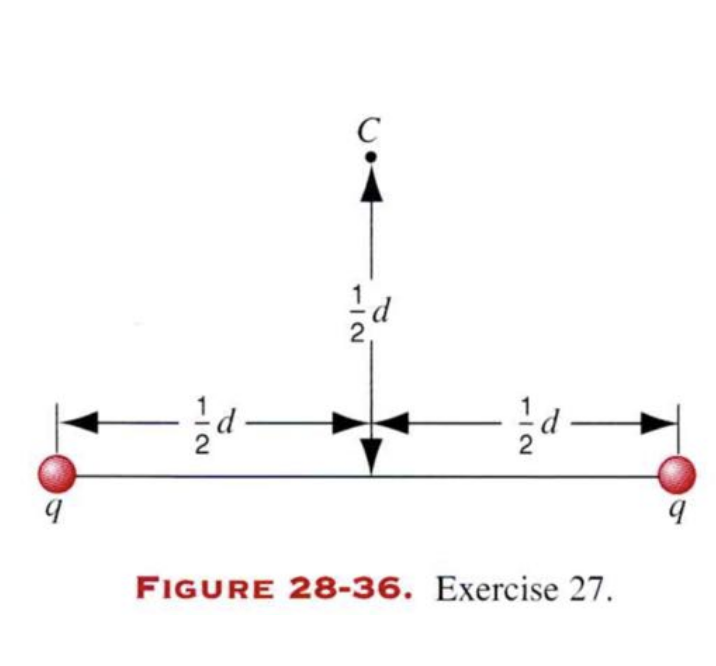
\includegraphics[scale=0.6]{28-36.png}
\end{center}
\end{problem}

\begin{solution}
\vfill
\end{solution}
\newpage

\begin{problem}[HRK P28.42]
Consider two widely separated conducting spheres, 1, and 2, the second having twice the diameter of the first. The smaller sphere initially has a positive charge $q$ and the larger one is initially uncharged. You now connect the spheres with a long  thin wire. $(a)$ How are the final potentials $V_1$ and $V_2$ of the spheres related? $(b)$ Find the charges $q_1$ and $q_2$ on the spheres in terms of $q$ 
\end{problem}

\begin{solution}
\vfill
\end{solution}
\newpage

\begin{problem}[5]
Consider a sphere of radius $R$ with a constant volume charge density $\rho$. Derive expressions for the electric field $ \vec{E}(r)$ and the electric potential $V(r)$ for all regions of space $r \leq R$ and $r \geq R$. Then sketch graphs of these functions aligned on the same $r$ scale. Let $V (\infty) = 0$
\end{problem}

\begin{solution}
\vfill
\end{solution}
\newpage

\begin{problem}[HRK E29.29]
Before Rutherford’s discovery of the atomic nucleus in 
1911, a prevalent model of the atom was J. J.Thomson’s ``plum pudding” model, consisting of negative electrons  distributed within a  diffuse uniform cloud of positive charge.  In this archaic model, a helium atom might look like this illustration, with a spherical cloud of radius $R$ and charge $+2Q$ enclosing two electrons of charge $–Q$ each. Using your results from Problem 5, find the net potential energy of the electrons and then determine the equilibrium spacing $x$ that minimizes the potential energy.  (Note:  An equivalent alternative to using$V(r)$from Problem 5 is to find the value of x for which the net force on the electrons is zero.) 
\begin{center}
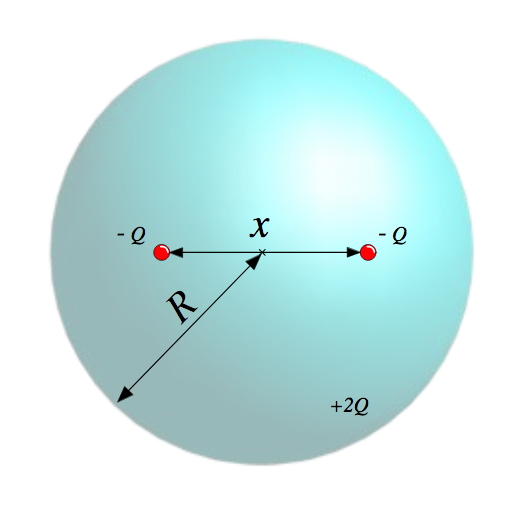
\includegraphics[scale=0.6]{Rutherford.png}
\end{center}
\end{problem}

\begin{solution}
\vfill
\end{solution}

\end{document}